\hypertarget{normal-subgroups-quotient-groups-and-homomorphisms}{%
\section{Normal Subgroups, Quotient groups and Homomorphisms}\label{normal-subgroups-quotient-groups-and-homomorphisms}}

Given a group \(G\), subgroup \(H\) of \(G\) and the set of left cosets of \(H\) in \(G\), \((G : H)\).
We would like to define a group operation on the cosets \(\circ\), so that \(((G : H), \circ)\) is a group.
Would like:
\begin{align*}
    (gH) \circ (k H) = gkH.
\end{align*}
When does this work?
Consider \(gH kH\) if \(Hk = kH\) then we get \(gkHH = gkH\).\\
This motivates the following definition.

\begin{definition}[Normal subgroup]
A subgroup \(K\) of \(G\) is called \emph{normal} if \(gK = Kg\) for all \(g \in G\).
We write \(K \trianglelefteq G\).
\end{definition}

\begin{example}
\begin{align*}
    K &= \{ \text{id}, \begin{pmatrix}1 & 2 & 3\end{pmatrix}, \begin{pmatrix}1 & 3 & 2\end{pmatrix} \} \trianglelefteq S_3 \\
    \begin{pmatrix}1 & 2\end{pmatrix} K &= \{ \begin{pmatrix}1 & 2\end{pmatrix}, \begin{pmatrix}2 & 3\end{pmatrix}, \begin{pmatrix}1 & 3\end{pmatrix} \} = K \begin{pmatrix}1 & 2\end{pmatrix} \\
    \begin{pmatrix}1 & 3\end{pmatrix} K &= K \begin{pmatrix}1 & 3\end{pmatrix} \\
    \begin{pmatrix}2 & 3\end{pmatrix} K &= K \begin{pmatrix}2 & 3\end{pmatrix} \\
    \begin{pmatrix}1 & 2 & 3\end{pmatrix} K &= K = K \begin{pmatrix}1 & 2 & 3\end{pmatrix}
\end{align*}
But \(H = \{ 1, \begin{pmatrix}1 & 2\end{pmatrix} \}\) is not normal in \(S_3\).
\begin{align*}
    \begin{pmatrix}1 & 3\end{pmatrix} H &= \{ \begin{pmatrix}1 & 3\end{pmatrix}, \begin{pmatrix}1 & 2 & 3\end{pmatrix} \} \\
    H \begin{pmatrix}1 & 3\end{pmatrix} &= \{ \begin{pmatrix}1 & 3\end{pmatrix}, \begin{pmatrix}1 & 3 & 2\end{pmatrix} \}
\end{align*}
\end{example}

\begin{proposition}
\protect\hypertarget{prp:four}{}\label{prp:four}

Let \(K \trianglelefteq G\).
TFAE (The following are equivalent):

\begin{enumerate}
\def\labelenumi{\roman{enumi}.}
\item
  \(gK = Kg \; \forall \; g \in G\)
\item
  \(gKg^{-1} = K \; \forall \; g \in G\)
\item
  \(gkg^{-1} \in K \; \forall \; k \in K,\ g \in G\)
\end{enumerate}

\end{proposition}

\begin{proof}
\begin{align*}
    (i) &\implies (ii) \\
    gKg^{-1} &= \{gkg^{-1} : k \in K \} \\
    &= (gK) g^{-1} \\
    &= (Kg)g^{-1} \\
    &= K.
\end{align*}

\((ii) \implies (iii)\)

\((iii) \implies (i)\) \\
For any \(k \in K,\ g \in G \; \exists \; k' \in K\) s.t. \(gkg^{-1} = k'\)
  \begin{align*}
    \implies gk &= k'g \in Kg \\
    \implies gK &\subseteq Kg \\
    \intertext{Similarly \(g^{-1}kg = k''\) for some \(k'' \in K\)}
    \implies kg &= gk'' \\
    \implies Kg &\subseteq gK \\
    \implies gK &= Kg.
  \end{align*}
\end{proof}

\begin{example} \mbox{}
  \begin{itemize}
  \item
    \(\{ e \} \trianglelefteq G,\ G \trianglelefteq G\).
  \item
    If \(G\) is abelian, all subgroups are normal.
    Since if \(k \in K,\ g \in G\) and \(K \leq G\) then \(gkg^{-1} = gg^{-1} k = k \in K\).
  \item
    Kernels of homomorphisms are normal subgroups (Sheet 1, q9) \(\implies A_n \trianglelefteq S_n\) since \(A_n = \ker sgn\)
  \item
    \(D_{2n} = \left\langle \underbrace{r,\ t}_\text{generators} | \underbrace{r^n = e,\ t^2 = e,\ trt = r^{-1}}_\text{relations} \right\rangle\).
    Then \(\langle r \rangle \trianglelefteq D_{2n}\).
    \begin{align*}
      \text{Clearly } r^i r^j r^{-i} &= r^j \in \langle r \rangle. \\
      \text{Also, } (r^i t) r^j (r^i t)^{-1} &= r^i t r^j t r^{-i} \\
      &= r^i r^{-j} t t r^{-i} \text{ as } tr^k = r^{-1}tr^{k-1} ... = r^{-k}t \\
      &= r^{-j} \in \langle r \rangle.
    \end{align*}
    Or use the following lemma.
  \end{itemize}
\end{example}

\begin{lemma}
\protect\hypertarget{lem:twelve}{}\label{lem:twelve}
If \(K \leq G\) and the index, \Cref{def:fourteen}, of \(K\) in \(G\) is 2, then \(K \trianglelefteq G\).
\end{lemma}

\begin{proof}
  \begin{align*}
      G &= K \mathbin{\dot{\cup}} gK \text{ for any } g \in G \setminus K 
      \intertext{as $g$ is in $gK$ but not $K$ so $gK \neq K$}
      &= K \mathbin{\dot{\cup}} Kg \text{ by \Cref{lem:ten}}
      \intertext{as $g$ is in $Kg$ but not $K$ so $Kg \neq K$}
      \implies gK &= Kg \; \forall \; g \in G, \text{ as if $g \in K$ then we just get $K = K$.}
  \end{align*} 
\end{proof}

\begin{theorem}
\protect\hypertarget{thm:five}{}\label{thm:five}
If \(K \trianglelefteq G\), the set \((G : K)\) of the left cosets of \(K\) in \(G\) is a group under coset multiplication i.e.~\(gK \circ hK = ghK\).\\
This group is called the \emph{quotient group} (or factor group) of \(G\) by \(K\) and denoted \(G / K\).
\end{theorem}

\begin{proof}
We need to check that coset multiplication is well defined.
\begin{align*}
    \text{i.e. } gK &= \hat{g}K \\
    \text{and } hK &= \hat{h}K \\
    \text{then } ghK &= \hat{g} \hat{h} K.
\end{align*}
By \Cref{lem:eleven},
\begin{align*}
    gK = \hat{g} K \implies \hat{g}^{-1} g &\in K \\
    hK = \hat{h} K \implies \hat{h}^{-1} h &\in K \\
    \text{Now } \hat{g}^{-1} g &\in K \\
    \implies h^{-1} \hat{g}^{-1} g h &\in K \text{ since } K \trianglelefteq G \\
    \implies (\hat{h}^{-1} h) (h^{-1} \hat{g}^{-1} g h) &\in K \\
    \implies \hat{h}^{-1}\hat{g}^{-1} g h &\in K \\
    \implies ghK &= \hat{g} \hat{h} K \text{ by \Cref{lem:eleven}.}
\end{align*} 

So coset multiplication is well-defined.
Group axioms now follow easily.

\begin{itemize}
\item
  By construction coset multiplication is closed as \(ghK \in (G : H)\) for \(g, h \in G\).
\item
  Identity given by \(eK = K\)
\item
  \((gK)^{-1} = g^{-1} K\)
\item
  Associativity holds since it does in \(G\), to check:
  \((gK hK) lK = (gh)l K = g(hl)K = gK (hK lK)\).
\end{itemize}

\end{proof}

\begin{example} \mbox{}
  \begin{enumerate}
  \def\labelenumi{\roman{enumi}.}
  \item
    \begin{align*}
      S_n / A_n &= \left( \left\{ A_n, \begin{pmatrix}1 & 2\end{pmatrix} A_n \right\}, \circ \right) \\
      &\cong C_2.
    \end{align*}
  \item
    \begin{align*}
      D_8 = \langle a, b : a^4 = e = b^2,\ bab = a^{-1} \rangle
      \end{align*}
      Let \(K = \{1, a^2 \}\).\\
      Claim: \(K \trianglelefteq D_8\).
      \begin{align*}
      (a^i b) a^2 (a^i b)^{-1} &= a^i b a^2 b a^{-i} \\
      &= a^i a^{-2} b b a^{-i} \text{ as } ba^2 = a^{-1}ba = a^{-2}b \\
      &= a^{-2} a^2 \in K \\
      a^i a^2 a^{-i} &= a^2 \in K. \\
      |D_8| / |K| &= 4 = |(D_8 : K)|.
      \intertext{$4$ distinct left cosets:}
      K &= \{ 1, a^2 \} \\
      aK &= \{ a, a^3 \} \\
      bK &= \{ b, ba^2 \} = \{ b, a^2 b \} \\
      abK &= \{ ab, aba^2 \} = \{ ab, a^3 b \}.
    \end{align*}
    %
    \begin{align*}
        \begin{array}{c|cccc}
            \circ & K & aK & bK & abK \\
            \hline
            K   & K   & aK   & bK  & abK \\
            aK  & aK  & K & abK & bK  \\
            bK  & bK  & abK  & K   & aK  \\
            abK & abK & bK   & aK  & K
        \end{array} 
    \end{align*}
    %
    Note \(aK aK = a^2 K = K\)
    This is isomorphic to \Cref{exm:nine}.
  \item
    Recall the subgroups of \((\mathbb{Z}, +)\) are precisely the groups \((n \mathbb{Z}, +)\) where \(n \in N \cup \{ 0 \}\), \(n \mathbb{Z} = \{ nk : k \in \mathbb{Z} \}\).
    Since \((\mathbb{Z}, +)\) is abelian, all subgroups are normal, \(n \mathbb{Z} \trianglelefteq Z\).\\
    Suppose \(n = 5\), cosets given by,
    \begin{align*}
        5 \mathbb{Z} &= \{ 5k : k \in \mathbb{Z} \} \\
        1 + 5 \mathbb{Z} &= \{ 1 + 5k : k \in \mathbb{Z} \} \\
        2 + 5 \mathbb{Z} &= \{ 2 + 5k : k \in \mathbb{Z} \} \\
        3 + 5 \mathbb{Z} &= \{ 3 + 5k : k \in \mathbb{Z} \} \\
        4 + 5 \mathbb{Z} &= \{ 4 + 5k : k \in \mathbb{Z} \}. \\
        (1 + 5 \mathbb{Z}) + (2 + 5 \mathbb{Z}) &= 3 + 5 \mathbb{Z}. \\
        (3 + 5 \mathbb{Z}) + (4 + 5 \mathbb{Z}) &= 2 + 5 \mathbb{Z}. \\
    \end{align*}
    %
    \emph{Claim}: \(( \mathbb{Z} / 5 \mathbb{Z}, \underbrace{\circ}_\text{coset \\ `addition'}) \cong \left( \{ 0, 1, 2, 3, 4 \}, +_5 \right)\)\footnote{It is coset `addition' as it is abelian}

    We define a map \(\theta : n + 5 \mathbb{Z} \to \overline{n}\) where \(n \equiv \overline{n} \mod 5\) and \(\overline{n} \in \{ 0, 1, 2, 3, 4 \}\).

    Well-defined map:
    \begin{align*}
        \text{if } n + 5 \mathbb{Z} &= m + 5 \mathbb{Z} \\
        \implies - m + n &\in 5 \mathbb{Z} \text{ by \Cref{lem:eleven}} \\
        \implies - m + n &\equiv 0 \pmod 5 \\
        \implies n &\equiv m \pmod 5 \\
        \implies \overline{n} &\equiv \overline{m}
        \intertext{homomorphism:}
        \theta\left( (n + 5 \mathbb{Z}) + (m + 5 \mathbb{Z}) \right) &= \theta( n + m + 5 \mathbb{Z}) \\
        &= \overline{n + m} \\
        &= \overline{n} +_5 \overline{m} \\
        &= \theta(n + 5 \mathbb{Z}) + \theta(m + 5 \mathbb{Z}).
    \end{align*}
    %
    In general \((\mathbb{Z} / n \mathbb{Z}, \circ) \cong \left( \{ 0, 1, \ldots, n - 1 \}, +_n \right)\).
  \end{enumerate}
\end{example} 

\medskip

Recall the definition of a homomorphism, \Cref{def:homomorphism}, \\
\(\operatorname{Im}(\theta) = \{ \theta (g) : g \in G \} \leq H\) (\Cref{lem:three}).
\(\ker(\theta) = \{ g \in G : \theta (g) = e_H \} \trianglelefteq G\) (Sheet 1).

\begin{theorem}[1st Isomorphism Theorem]
\protect\hypertarget{thm:six}{}\label{thm:six}
Let \(G, H\) be groups and \(\theta : G \to H\) a group homomorphism.
Then \begin{align*}
    \operatorname{Im} \theta &\leq H \\
    \ker \theta &\trianglelefteq G \\
    \text{and } G / \ker \theta &\cong \operatorname{Im} \theta.
\end{align*}
\end{theorem}

\begin{definition}[Simple group]
\protect\hypertarget{def:sixteen}{}\label{def:sixteen}
A group is called \emph{simple} if its only normal subgroups are \(\{ e \}\) and \(G\),
e.g.~\(C_p\) where \(p\) is prime.
\end{definition}

\begin{center}\rule{\linewidth}{0.5pt}\end{center}

\emph{Aside}

\begin{definition}
  Suppose \(f : A \to B\)

  \begin{enumerate}
  \def\labelenumi{\roman{enumi}.}
  \item
    \(f\) is \emph{injective} (one-to-one) if \(a_1, a_2 \in A\), \(f(a_1) = f(a_2) \implies a_1 = a_2\) (each element of \(A\) maps to a different element of \(B\)).
  \item
    \(f\) is \emph{surjective} (onto) if given \(b \in B \; \exists \; a \in A\) such that \(f(a) = b\) (every element in \(B\) is `hit').
  \item
    \(f\) is \emph{bijective} if \(f\) is both injective and surjective.
  \end{enumerate}
\end{definition}

\begin{center}\rule{\linewidth}{0.5pt}\end{center}

\begin{proof}[Proof (1st Isomorphism Theorem).]
Let $K = \ker \theta$, we need to construct an isomorphism
\begin{align*}
    \phi : G / \ker \theta &\to \operatorname{Im} \theta \\
    \ gK &\mapsto \theta(g).
\end{align*}

{\centering 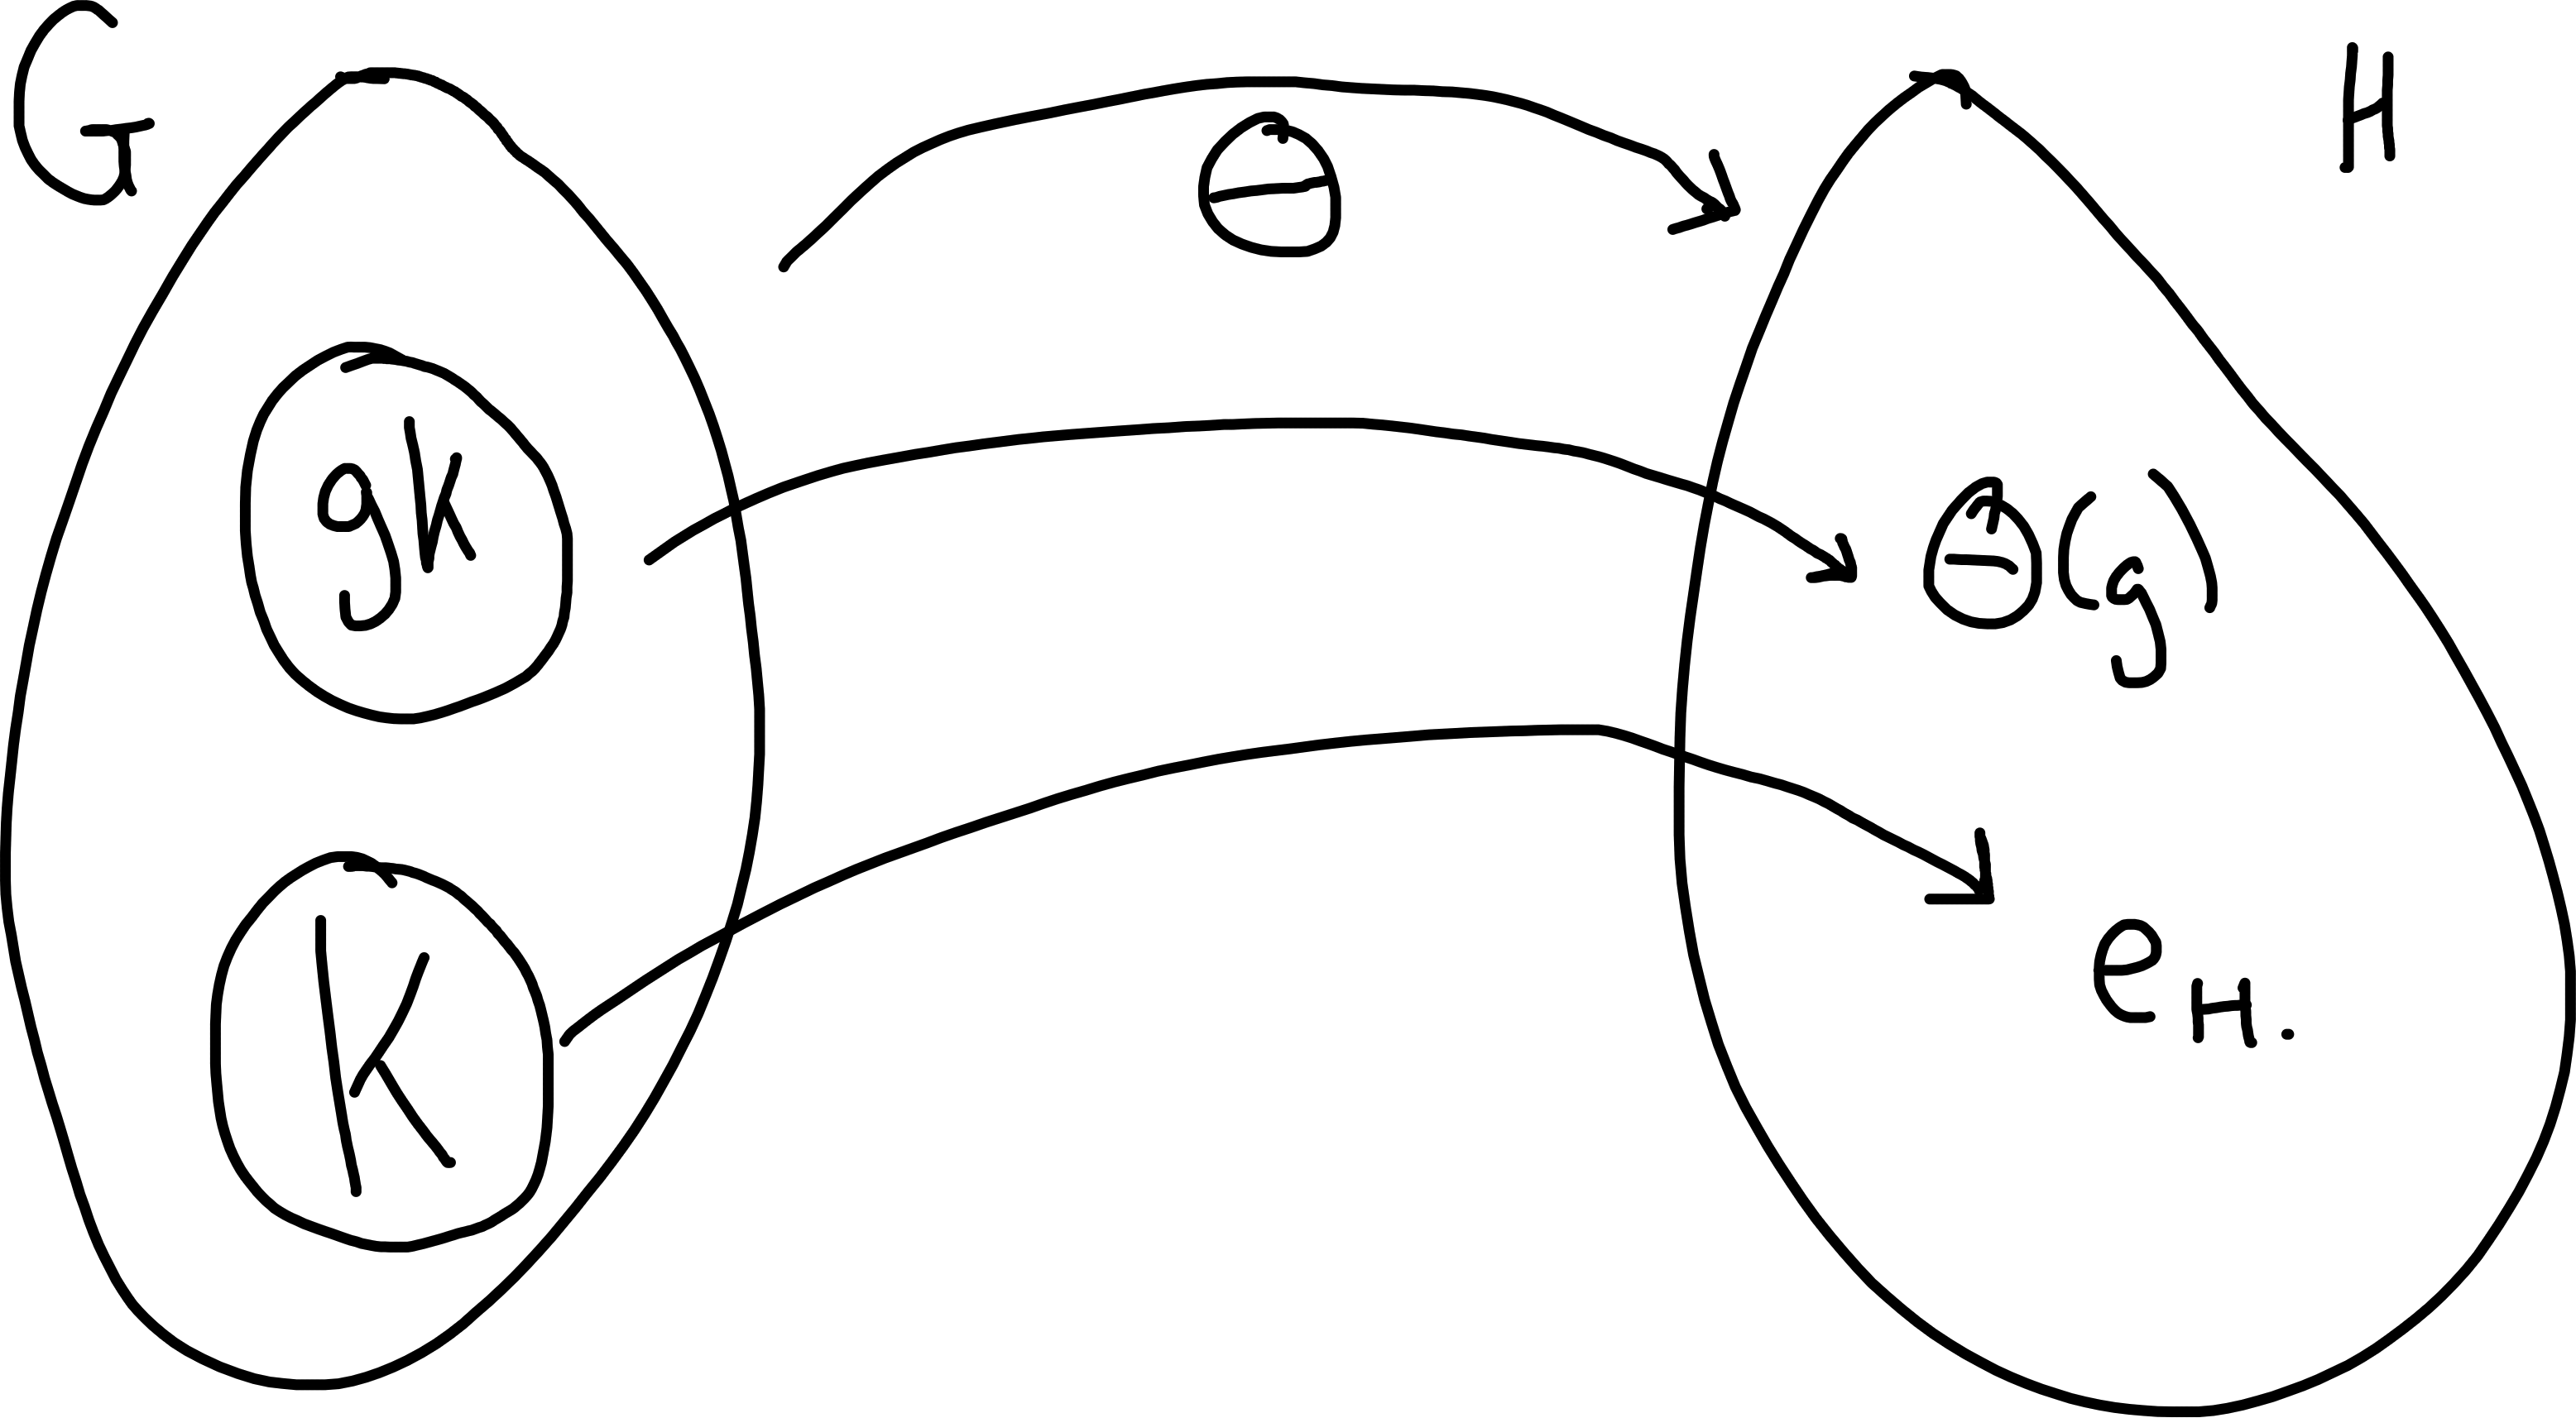
\includegraphics[height=5cm]{figures/04-iso-thm}}

Need \(\phi\) well-defined:
\begin{align*}
    \text{Suppose } gK &= hK \\
    \implies h^{-1}g &\in K \text{ see \Cref{lem:eleven}} \\
    \implies \theta(h^{-1}g) &= e_H \\
    \theta(h)^{-1} \theta(g) &= e_H \text{ since $\theta$ is a homomorphism} \\
    \implies \theta(g) &= \theta(h) \\
    \implies \phi(gK) &= \phi(hK)
\end{align*}
%
Need \(\phi\) to be a homomorphism:
\begin{align*}
    \phi(gK hK) &= \phi(gh K) \\
    &= \theta(gh) \\
    &= \theta(g) \theta(h) \text{ since $\theta$ is a homomorphism} \\
    &= \phi(gK) \phi(hK).
\end{align*}
%
\(\phi\) surjective:
If \(\theta(g) \in \operatorname{Im} \theta\) then \(\phi(gK) = \theta(g)\).

\(\phi\) injective:
Suppose \(\phi(gK) = \phi(hK)\)
\begin{align*}
    \text{Suppose } \phi(gK) &= \phi(hK) \\
    \implies \theta(g) &= \theta(h) \\
    \implies \theta(h)^{-1} \theta(g) &= e_H \\
    \theta(h^{-1}g) &= e_H \\
    \implies h^{-1} g &\in K \\
    \implies gK &= hK. 
\end{align*}
\end{proof}

\begin{remark}
  By the \nameref{thm:six}, $\operatorname{Im} \theta \cong G / \ker \theta$, a homomorphic image of $G$ is isomorphic to a quotient of $G$. 
\end{remark}

\hypertarget{examples}{%
\subsection{Examples}\label{examples}}

\begin{example}
\begin{align*}
    \operatorname{sgn} : S_n &\to ( \{ \pm 1 \}, \times) \\
    \sigma &\mapsto \operatorname{sgn}(\sigma). \\
    \operatorname{Im}(\text{sgn}) &= ( \{ \pm 1 \}, \times) \\
    \ker(\text{sgn}) &= A_n \\
    \implies S_n / A_n &\cong ( \{ \pm 1 \}, \times) \cong C_2 \\
    \implies |A_n| &= \frac{|S_n|}{2}
\end{align*}
\end{example}

\begin{example}
\begin{align*}
    \theta : (\mathbb{R}, +) &\to (\mathbb{C} \setminus \{ 0 \}, \times) \\
    r &\mapsto e^{2 \pi i r} \\
    \text{Note, } \theta(r + s) &= \theta(r) \theta(s) \\
    \operatorname{Im}(\theta) &= S^1 = \{ z \in \mathbb{C} : |z| = 1 \} \text{ unit circle} \\
    \ker (\theta) &= (\mathbb{Z}, +) \trianglelefteq  (\mathbb{R}, +) . \\
    (\mathbb{R}, +) / (\mathbb{Z}, +) &\cong S^1.
\end{align*}
\end{example}

\begin{example}
Recall \cref{exm:glg} and \ref{exm:sltwo}.
\begin{align*}
    GL_2 (\mathbb{R}) &= \{ 2 \times 2 \text{ matrices with entries in } \mathbb{R}, \det \neq 0 \}. \\
    \det : GL_2 (\mathbb{R}) &\to (\mathbb{R} \setminus, \{0 \}, \times) \\
    M &\mapsto \det (M) \\
    \det (AB) &= \det A \det B \text{ so is a homomorphism}. \\
    \operatorname{Im} \det &= (\mathbb{R} \setminus \{ 0 \}, \times) \\
    \text{since } \det \begin{pNiceMatrix}
      \alpha   &       & \Block{2-3}<\huge>{0} \\
          &   1   &        &      &       \\
          &       &   1    &      &       \\
      \Block{2-3}<\huge>{0}
          &       &       & \Ddots    &   \\
          &       &       &      &   1   \\
    \end{pNiceMatrix} &= \alpha \in \mathbb{R} \setminus \{ 0 \} \\
    \ker \det &= \mathrm{SL}_2 (\mathbb{R}) = \{ 2 \times 2 \text{ matrices with entries in } \mathbb{R}, \det = 1 \}. \\
    \implies \mathrm{SL}_2(\mathbb{R}) &\trianglelefteq GL_2(\mathbb{R}) \\
    \text{and } GL_2 (\mathbb{R}) / \mathrm{SL}_2 (\mathbb{R}) &\cong ( \mathbb{R} \setminus \{ 0 \}, \times)
\end{align*}
\end{example}

\begin{example}
\begin{align*}
    \theta : (\mathbb{Z}, +) &\to ( \{ 0, 1, \ldots, n-1), +_n) \\
    n &\mapsto \overline{n} \\
    \ker \theta &= n \mathbb{Z}.
\end{align*}
\end{example}

\begin{lemma}
  Given $K \trianglelefteq G$, the \emph{quotient map} $q: G\rightarrow G/K$ with $g\mapsto gK$ is a surjective group homomorphism.
\end{lemma}

\begin{proof}
  $q(ab) = (ab)K = aKbK = q(a)q(b)$. So $q$ is a group homomorphism. Also for all $aK \in G/K$, $q(a) = aK$. So it is surjective.
\end{proof}

Note that the kernel of the quotient map is $K$ itself.

\begin{lemma}
\protect\hypertarget{lem:thirteen}{}\label{lem:thirteen}A homomorphism \(\theta : G \to H\) is injective iff \(\ker \theta = \{ e_G \}\).
\end{lemma}

\begin{proof}
(\(\implies\)): Suppose \(\theta(g) = e_H = \theta (e_G)\).
So injectivity \(\implies g = e_G\).

(\(\Longleftarrow\)): \begin{align*}
    \theta(g) &= \theta(h) \\
    \implies \theta(h)^{-1} \theta(g) &= e_H \\
    \implies \theta(h^{-1} g) &= e_H \\
    \implies h^{-1} g \in \ker \theta &= \{ e_G \} \\
    \implies h^{-1} g &= e_G \\
    \implies h &= g.
\end{align*}
\end{proof}

\begin{align*}
    \text{Recall if } N \trianglelefteq G, g \in G, n \in N \\
    \implies gng^{-1} \in N \\
    \implies gng^{-1} = \hat{n} \text{ for some } \hat{n} \in N \\
    \implies gn = \hat{n} g.
\end{align*}
This allows us to reorder our elements and helps in proving the following lemma.

\begin{lemma}
\protect\hypertarget{lem:fourteen}{}\label{lem:fourteen}
\mbox{}
  \begin{enumerate}
  \def\labelenumi{\roman{enumi}.}
  \item
    Let \(N \trianglelefteq G, H \leq G\).
    Then \(NH = \{ nh : n \in N, h \in H \} \leq G\).
  \item
    Let \(N \trianglelefteq G, M \trianglelefteq G\) then \(NM \trianglelefteq G\).
  \end{enumerate}
\end{lemma}

\begin{proof} \mbox{}
  \begin{enumerate} \def\labelenumi{\roman{enumi}.}
  \item
    Closure, \(nh, \overline{n} \overline{h} \in NH\)
    \begin{align*}
      n \underbrace{h \overline{n}}_{\hat{n} h} \overline{h} = n \hat{n} h \overline{h} \in NH
    \end{align*}

    \(\text{id} = e = \exists \in NH\)

    inverse:
    \begin{align*}
        (nh)^{-1} &= h^{-1} n^{-1} \\
        &= \hat{n} h^{-1} \text{ for some } \hat{n} \in N. \\
        &\in NH
    \end{align*}
    %
  \item
    we need to check normality
    \begin{align*}
      g (nm) g^{-1} &= \underbrace{g n g^{-1}}_{\in N} \underbrace{g m g^{-1}}_{\in M} \in NM.\\
    \end{align*}
  \end{enumerate}
\end{proof}